\documentclass[aspectratio=169,12pt,t]{beamer}

% --- Theme: Metropolis (modern, clean) ---
\usetheme[progressbar=frametitle,numbering=fraction,block=fill]{metropolis}

% --- Fira Sans font (install texlive-fonts-extra if missing) ---
\IfFileExists{FiraSans.sty}{\usepackage[sfdefault]{FiraSans}}{}

% --- Light background with warm accent ---
\definecolor{mDarkTeal}{RGB}{35,55,59}
\definecolor{mLightBrown}{RGB}{235,228,216}
\definecolor{mAccent}{RGB}{140,70,20}

\setbeamercolor{normal text}{fg=mDarkTeal,bg=white}
\setbeamercolor{alerted text}{fg=mAccent}
\setbeamercolor{frametitle}{bg=mDarkTeal,fg=white}
\setbeamercolor{progress bar}{fg=mAccent,bg=mLightBrown}
\setbeamercolor{title separator}{fg=mAccent}
\setbeamercolor{progress bar in head/foot}{fg=mAccent,bg=mLightBrown}
\setbeamercolor{progress bar in section page}{fg=mAccent,bg=mLightBrown}

% --- Packages ---
\usepackage[utf8]{inputenc}
\usepackage{amsmath,amssymb,amsthm}
\usepackage{mathrsfs}
\usepackage{tikz}
\usetikzlibrary{arrows.meta,positioning,calc,decorations.pathreplacing,shapes,patterns}
\usepackage{pgfplots}
\pgfplotsset{compat=1.18}

% --- Semi-transparent white highlight for text on top of background images ---
\usepackage[most]{tcolorbox}

% Inline highlight: \hl{short text}
\newtcbox{\hl}{%
  nobeforeafter, tcbox raise base,
  colback=white, opacityback=0.6,
  colframe=white, opacityframe=0,
  sharp corners, boxsep=2pt, left=3pt, right=3pt, top=2pt, bottom=2pt%
}

% Block highlight: \begin{hlbox} ... \end{hlbox}  (multi-line, paragraphs, itemize)
\newtcolorbox{hlbox}[1][]{%
  enhanced, breakable,
  colback=white, opacityback=0.6,
  colframe=white, opacityframe=0,
  boxsep=3pt, left=6pt, right=6pt, top=4pt, bottom=4pt,
  sharp corners,
  {#1}%
}

% --- Custom colors for content types ---
\definecolor{defcolor}{RGB}{25,85,120}
\definecolor{thmcolor}{RGB}{140,35,35}
\definecolor{proofcolor}{RGB}{35,100,50}
\definecolor{excolor}{RGB}{140,75,10}
\definecolor{remcolor}{RGB}{90,90,90}

% --- Beamer blocks for mathematical content types (semi-transparent) ---
\tcbset{hlblockbase/.style={
  enhanced, breakable,
  coltitle=white, fonttitle=\bfseries,
  opacitybacktitle=0.8, opacityback=0.6,
  opacityframe=0,
  sharp corners,
  boxsep=1pt, left=5pt, right=5pt, top=2pt, bottom=2pt,
  toptitle=1pt, bottomtitle=1pt
}}

\newtcolorbox{defblock}[1]{hlblockbase, title={#1},
  colbacktitle=defcolor, colback=defcolor!15, colframe=defcolor}
\newtcolorbox{thmblock}[1]{hlblockbase, title={#1},
  colbacktitle=thmcolor, colback=thmcolor!15, colframe=thmcolor}
\newtcolorbox{proofblock}[1]{hlblockbase, title={#1},
  colbacktitle=proofcolor, colback=proofcolor!15, colframe=proofcolor}
\newtcolorbox{exblock}[1]{hlblockbase, title={#1},
  colbacktitle=excolor, colback=excolor!15, colframe=excolor}
\newtcolorbox{remblock}[1]{hlblockbase, title={#1},
  colbacktitle=remcolor, colback=remcolor!15, colframe=remcolor}

% --- Metadata ---
\title{Chapter 3: Numerical Sequences and Series}
\subtitle{Section: Power Series}
\author{Based on Walter Rudin's \emph{Principles of Mathematical Analysis}}
\date{}

\begin{document}

% =============================================================================
% TITLE AND OUTLINE
% =============================================================================
{
\usebackgroundtemplate{%
  
\includegraphics[width=\paperwidth,height=\paperheight,keepaspectratio=false]{chapter_03_bg_00.png}%
}
\begin{frame}[plain]
  \titlepage
  \note{
    Welcome back to Chapter 3 of Principles of Mathematical Analysis. In
    this short but important section we meet power series. A power series
    is an infinite sum built from powers of a complex variable "z", with
    fixed coefficients. These are the building blocks of analysis: the
    exponential function, the sine and cosine, and countless others are
    all defined by power series. Our central question is simple to state.
    For which values of "z" does the series converge? The answer is
    beautifully clean. There is a single number "R", the radius of
    convergence, computed directly from the coefficients by the root
    test. Inside a disk of radius "R" the series converges; outside it
    diverges. Let's see how this works.
  }
\end{frame}
}

{
\usebackgroundtemplate{%
  
\includegraphics[width=\paperwidth,height=\paperheight,keepaspectratio=false]{chapter_03_bg_01.png}%
}
\begin{frame}[c]{Outline}
  \begin{center}
    \tableofcontents
  \end{center}
  \note{
    Here is our plan. We start with motivation, recalling why power
    series matter and what question we are trying to answer. Then we give
    the formal definition of a power series and introduce the circle of
    convergence. Next comes the main theorem, which pins down the radius
    of convergence using the root test, together with its short proof.
    After that we work through five examples that show every possible
    kind of behavior. Finally we summarize the key ideas.
  }
\end{frame}

% =============================================================================
\section{Motivation}
% =============================================================================

% --- Build 1/3 ---
\begin{frame}{Why Power Series Matter}
  \begin{hlbox}
    \begin{itemize}
      \item Many key functions are \alert{defined} by power series:
        $\displaystyle e^z = \sum_{n=0}^{\infty}\frac{z^n}{n!}$
    \end{itemize}
  \end{hlbox}

  \note{
    Let's start with why these objects deserve a section of their own.
    Many of the most important functions in all of mathematics are not
    given by simple formulas; instead, they are defined by power series.
    The exponential function shown on the slide is the prime example. It
    is literally defined as the infinite sum of "z" to the "n" over "n"
    factorial. The same is true of the sine, the cosine, and the
    logarithm. Next, let's see what makes a power series usable.
  }
\end{frame}

% --- Build 2/3 ---
\begin{frame}{Why Power Series Matter}
  \begin{hlbox}
    \begin{itemize}
      \item Many key functions are \alert{defined} by power series:
        $\displaystyle e^z = \sum_{n=0}^{\infty}\frac{z^n}{n!}$
      \item A power series only makes sense where it \alert{converges}
    \end{itemize}
  \end{hlbox}

  \note{
    But there is a catch. An infinite sum is only meaningful where it
    actually converges to a finite value. So before we can treat a power
    series as a function, we must know exactly which values of "z" make
    the series add up. For some series that is every "z", for others only
    a few. Next, let's state the question precisely.
  }
\end{frame}

% --- Build 3/3 ---
\begin{frame}{Why Power Series Matter}
  \begin{hlbox}
    \begin{itemize}
      \item Many key functions are \alert{defined} by power series:
        $\displaystyle e^z = \sum_{n=0}^{\infty}\frac{z^n}{n!}$
      \item A power series only makes sense where it \alert{converges}
      \item Central question: \alert{for which $z$ does $\sum c_n z^n$ converge?}
    \end{itemize}
  \end{hlbox}

  \note{
    This is the central question of the section. Given the coefficients
    "c" sub "n", for which complex numbers "z" does the series of "c" sub
    "n" times "z" to the "n" converge? Remarkably, the answer has a very
    clean shape. The set of good "z" is essentially a disk in the complex
    plane, and its radius can be read straight off the coefficients.
    Let's make all of this precise.
  }
\end{frame}

}

{
\usebackgroundtemplate{%
  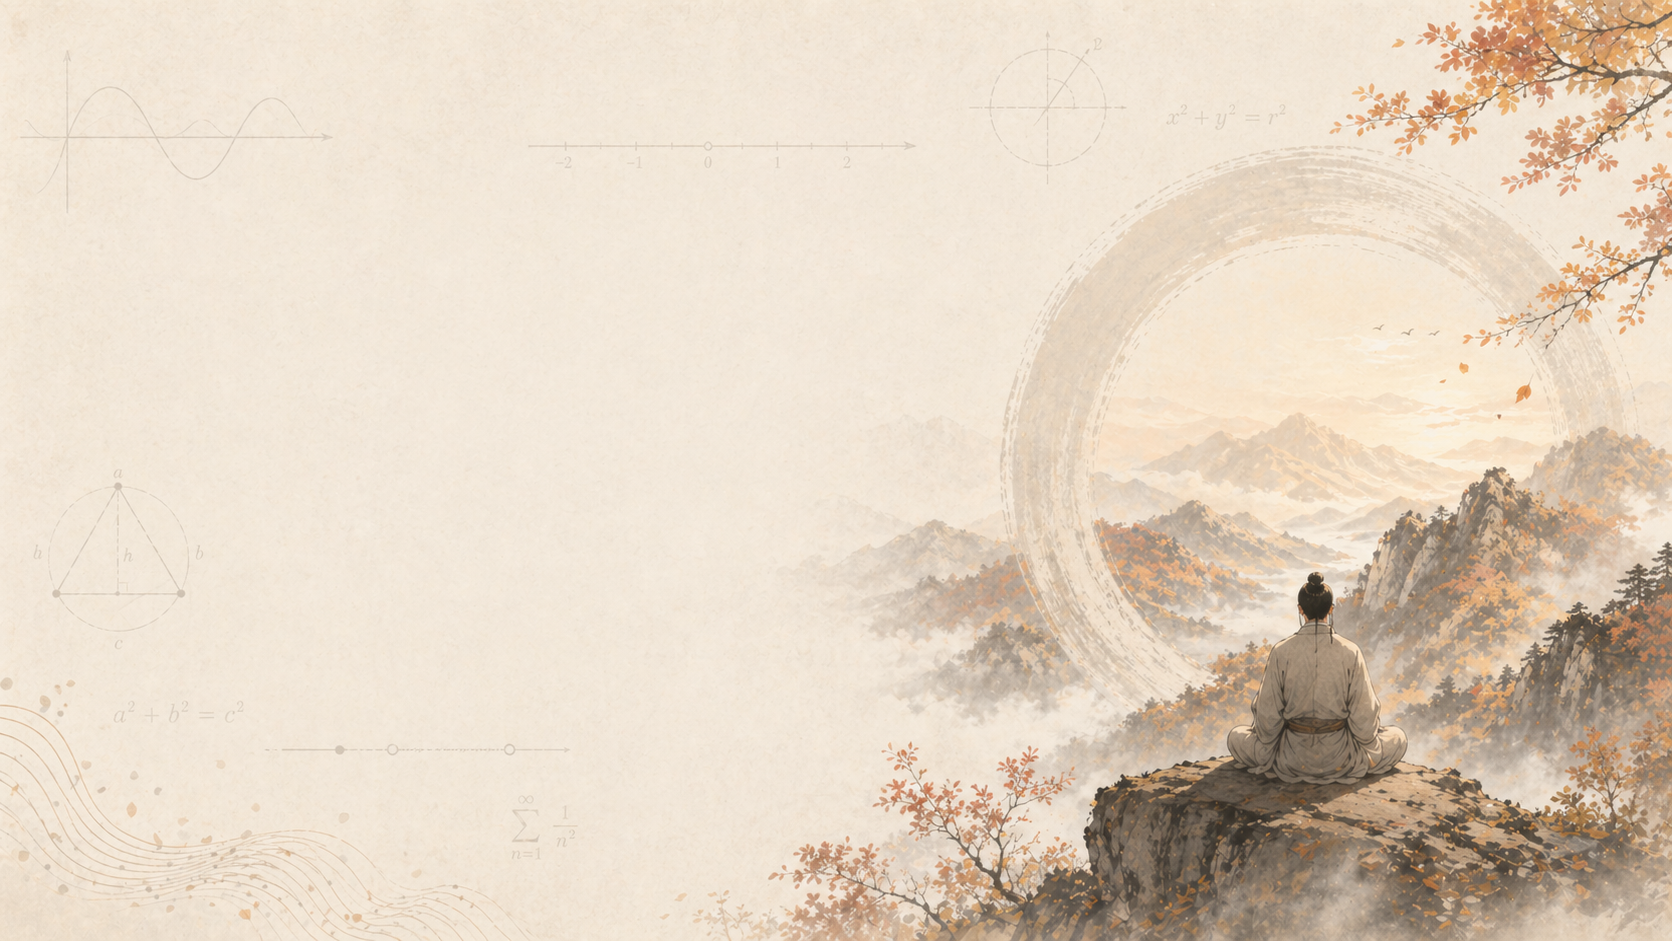
\includegraphics[width=\paperwidth,height=\paperheight,keepaspectratio=false]{chapter_03_bg_02.png}%
}
% =============================================================================
\section{Definition}
% =============================================================================

\begin{frame}{Definition 3.38: Power Series}
  \begin{defblock}{Definition 3.38}
    Given a sequence $\{c_n\}$ of complex numbers, the series
    \[
      \sum_{n=0}^{\infty} c_n z^n
    \]
    is called a \alert{power series}. The numbers $c_n$ are the
    \emph{coefficients}; $z$ is a complex number.
  \end{defblock}

  \vspace{0.4em}
  \hl{\textbf{Key point:} convergence depends on the choice of $z$.}

  \note{
    Here is the formal definition. We are handed a sequence of complex
    numbers "c" sub "n", the coefficients, and "z" is a complex variable.
    The power series is the infinite sum, from "n" equals zero to
    infinity, of "c" sub "n" times "z" to the "n". Notice that the sum
    starts at "n" equals zero, so the very first term is just the constant
    "c" sub zero. We allow "z" to be complex, not merely real, because
    that is the natural setting in which this theory becomes clean and
    symmetric, as we will see in a moment. The key point, stated at the
    bottom of the slide, is that whether this series converges depends
    entirely on which "z" we plug in. The very same coefficients can give
    a series that converges for one choice of "z" and diverges for
    another. Next, let's picture the set of "z" where it converges.
  }
\end{frame}

\begin{frame}{The Circle of Convergence}
  \begin{columns}[c]
    \begin{column}{0.52\textwidth}
      \begin{remblock}{Geometric picture}
        Every power series has an associated \alert{circle of convergence}
        of radius $R$:
        \begin{itemize}
          \item converges if $z$ is \alert{inside}
          \item diverges if $z$ is \alert{outside}
          \item on the circle: \emph{varies}
        \end{itemize}
      \end{remblock}
    \end{column}
    \begin{column}{0.48\textwidth}
      \begin{center}
      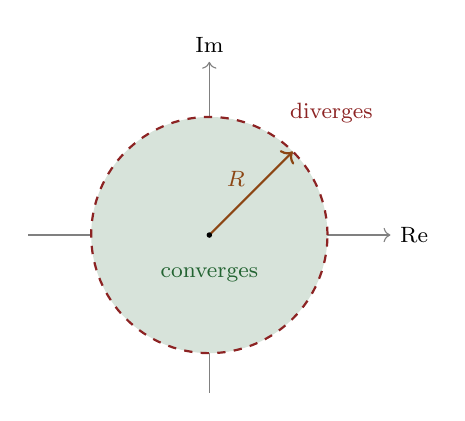
\begin{tikzpicture}[scale=1.0]
        % axes
        \draw[->,gray] (-2.3,0) -- (2.3,0) node[right,black]{\footnotesize Re};
        \draw[->,gray] (0,-2.0) -- (0,2.2) node[above,black]{\footnotesize Im};
        % converging disk
        \fill[proofcolor!18] (0,0) circle (1.5);
        \draw[thick,dashed,thmcolor] (0,0) circle (1.5);
        % radius
        \draw[->,thick,mAccent] (0,0) -- (1.06,1.06) node[midway,above left=-2pt]{\footnotesize $R$};
        \node[proofcolor] at (0,-0.5) {\footnotesize converges};
        \node[thmcolor] at (1.55,1.55) {\footnotesize diverges};
        \fill (0,0) circle (1pt);
      \end{tikzpicture}
      \end{center}
    \end{column}
  \end{columns}

  \note{
    On the slide is the geometric picture that organizes everything. With
    every power series we associate a circle in the complex plane,
    centered at the origin, called the circle of convergence. Its radius
    is "R". In the diagram, the green shaded disk is where the series
    converges, the inside of the circle, while everything outside the
    dashed red circle is where it diverges. The orange arrow marks the
    radius "R". Now, why should the good region be a perfect disk in the
    first place? The reason is simple but important. The size of each term,
    the absolute value of "c" sub "n" times "z" to the "n", equals the
    absolute value of "c" sub "n" times the absolute value of "z" raised
    to the "n". So a term's magnitude depends on "z" only through its
    distance from the origin, never its direction. Convergence can
    therefore depend only on that distance, and that is exactly what carves
    out a circle. On the circle itself the behavior is delicate and can go
    either way, so we leave that boundary case aside for now. At the
    extremes, the disk may have infinite radius, meaning convergence
    everywhere, or radius zero, meaning the origin only. Next, the theorem
    that computes "R".
  }
\end{frame}

}

{
\usebackgroundtemplate{%
  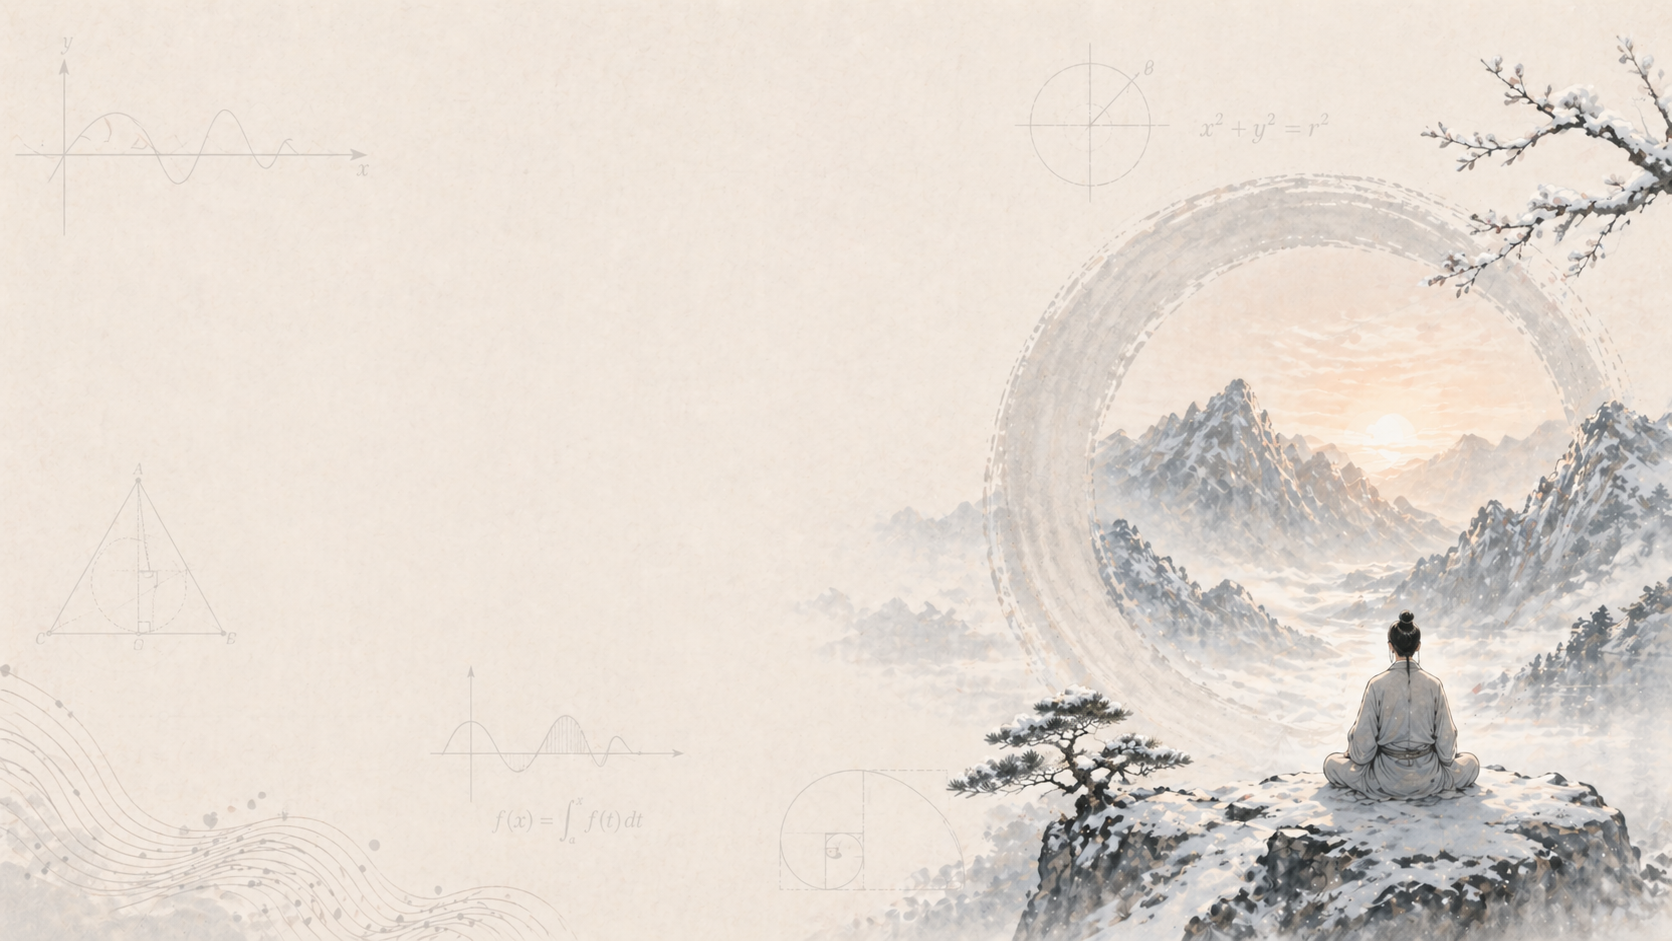
\includegraphics[width=\paperwidth,height=\paperheight,keepaspectratio=false]{chapter_03_bg_03.png}%
}
% =============================================================================
\section{The Radius of Convergence}
% =============================================================================

\begin{frame}{Theorem 3.39: Radius of Convergence}
  \begin{thmblock}{Theorem 3.39}
    Given $\sum c_n z^n$, put
    \[
      \alpha = \limsup_{n\to\infty} \sqrt[n]{|c_n|},
      \qquad R = \frac{1}{\alpha}.
    \]
    Then $\sum c_n z^n$ \alert{converges if $|z| < R$} and
    \alert{diverges if $|z| > R$}.
  \end{thmblock}

  \vspace{0.3em}
  \begin{remblock}{Edge cases}
    If $\alpha = 0$, then $R = +\infty$; \quad if $\alpha = +\infty$, then $R = 0$.
  \end{remblock}

  \note{
    Here is the main theorem, and it is wonderfully concrete. We form the
    quantity alpha, the limit superior of the "n"th root of the absolute
    value of "c" sub "n". Why the limit superior, rather than an ordinary
    limit? Because the plain limit might fail to exist if the coefficients
    behave irregularly, but the limit superior always exists, so alpha is
    always well defined. Notice it depends only on the coefficients, not on
    "z". Then "R", the radius, is simply one over alpha. The conclusion
    matches the picture from before: the series converges whenever the
    absolute value of "z" is less than "R", and diverges whenever it is
    greater. The remark handles the two extreme cases. If alpha is zero, we
    set "R" to plus infinity, so the series converges everywhere. If alpha
    is infinite, then "R" is zero, and the series converges only at the
    origin. Next comes the proof, which is just one line.
  }
\end{frame}

\begin{frame}{Proof of Theorem 3.39}
  \hl{\textbf{Strategy:} apply the \alert{root test} (3.33) to $a_n = c_n z^n$.}

  \vspace{0.5em}
  \begin{proofblock}{One line}
    \[
      \limsup_{n\to\infty}\sqrt[n]{|a_n|}
      = |z|\,\limsup_{n\to\infty}\sqrt[n]{|c_n|}
      = \frac{|z|}{R}.
    \]
    Root test: converges if $\dfrac{|z|}{R} < 1$, diverges if $\dfrac{|z|}{R} > 1$.
  \end{proofblock}

  \vspace{0.3em}
  \begin{center}
    \hl{$\boxed{|z| < R \Rightarrow \text{converges}, \qquad |z| > R \Rightarrow \text{diverges}.}$}
  \end{center}

  \note{
    The proof is a direct application of the root test from earlier in
    the chapter. We set "a" sub "n" equal to "c" sub "n" times "z" to the
    "n", the actual terms of our series. The "n"th root of the absolute
    value of "a" sub "n" factors cleanly: the absolute value of "z" comes
    out as a constant, leaving the "n"th root of the absolute value of "c"
    sub "n". Taking the limit superior turns that second factor into
    alpha, so the whole thing equals the absolute value of "z" divided by
    "R". The root test then says: converges when this quantity is below
    one, diverges when it is above one. Multiplying through by "R" gives
    exactly the statement of the theorem. The number "R" is called the
    radius of convergence. Next, let's see it in action.
  }
\end{frame}

}

{
\usebackgroundtemplate{%
  
\includegraphics[width=\paperwidth,height=\paperheight,keepaspectratio=false]{chapter_03_bg_04.png}%
}
% =============================================================================
\section{Examples}
% =============================================================================

\begin{frame}{Example 3.40(a): $R = 0$}
  \begin{exblock}{Example 3.40(a)}
    \[
      \sum n^n z^n \qquad\Longrightarrow\qquad R = 0.
    \]
  \end{exblock}

  \vspace{0.5em}
  \begin{hlbox}
    Here $\sqrt[n]{|c_n|} = \sqrt[n]{n^n} = n \to \infty$, so $\alpha = +\infty$
    and $R = 0$.

    \vspace{0.3em}
    \textbf{Meaning:} converges \alert{only at $z = 0$}.
  \end{hlbox}

  \note{
    Our first example is the series with coefficients "n" to the "n".
    Here the "n"th root of the absolute value of the coefficient is the
    "n"th root of "n" to the "n", which is just "n". As "n" grows, that
    runs off to infinity, so alpha is infinite and the radius "R" is zero.
    The meaning is that this power series converges only at the single
    point "z" equals zero, and nowhere else. The coefficients grow far too
    fast for any nonzero "z" to be tamed. Next, the opposite extreme.
  }
\end{frame}

\begin{frame}{Example 3.40(b): $R = +\infty$}
  \begin{exblock}{Example 3.40(b)}
    \[
      \sum \frac{z^n}{n!} \qquad\Longrightarrow\qquad R = +\infty.
    \]
  \end{exblock}

  \vspace{0.5em}
  \begin{hlbox}
    The ratio test is easier here: $\dfrac{|z|^{n+1}/(n+1)!}{|z|^n/n!}
    = \dfrac{|z|}{n+1} \to 0$ for every $z$.

    \vspace{0.3em}
    \textbf{Meaning:} converges for \alert{all $z$} --- this is $e^z$.
  \end{hlbox}

  \note{
    Now the opposite extreme. Take the coefficients to be one over "n"
    factorial. Here it is easier to use the ratio test than the root test.
    The ratio of consecutive terms is the absolute value of "z" divided by
    "n" plus one, and for any fixed "z" that goes to zero as "n" grows. A
    ratio with limit zero, which is below one, means convergence for every
    single "z". So the radius is infinite. This series is exactly the
    exponential function we met in the motivation. Next, the borderline
    case where the radius is one.
  }
\end{frame}

\begin{frame}{Example 3.40(c): $R = 1$, diverges on the circle}
  \begin{exblock}{Example 3.40(c)}
    \[
      \sum z^n \qquad\Longrightarrow\qquad R = 1.
    \]
  \end{exblock}

  \vspace{0.4em}
  \begin{hlbox}
    On the circle $|z| = 1$: the series \alert{diverges}, since $\{z^n\}$
    does not tend to $0$.
  \end{hlbox}

  \note{
    This is the plain geometric series, with all coefficients equal to
    one. The "n"th root of one is one, so alpha is one and the radius is
    one. The new feature here is the behavior on the boundary circle,
    where the absolute value of "z" equals one. There the series diverges
    at every point, because the terms "z" to the "n" all have absolute
    value one and never shrink toward zero. Recall that a series whose
    terms do not go to zero cannot converge. So on this circle, divergence
    is total. Next, a series that diverges at only one boundary point.
  }
\end{frame}

\begin{frame}{Example 3.40(d): $R = 1$, diverges only at $z = 1$}
  \begin{exblock}{Example 3.40(d)}
    \[
      \sum \frac{z^n}{n} \qquad\Longrightarrow\qquad R = 1.
    \]
  \end{exblock}

  \vspace{0.4em}
  \begin{hlbox}
    On the circle $|z| = 1$:
    \begin{itemize}
      \item \alert{diverges} at $z = 1$ (harmonic series)
      \item \alert{converges} at all other $z$ with $|z| = 1$ (Theorem 3.44)
    \end{itemize}
  \end{hlbox}

  \note{
    Now divide by "n". The "n"th root of one over "n" still tends to one,
    so again the radius is one. But the boundary behavior is now subtle
    and mixed. At the single point "z" equals one, the series becomes the
    harmonic series, one plus one half plus one third and so on, which
    diverges. Yet at every other point on the circle the series actually
    converges. That last fact is not obvious; it will be proved later
    using a tool called summation by parts, in Theorem 3.44. So here the
    circle has exactly one bad point. Next, a series that behaves
    perfectly on the entire circle.
  }
\end{frame}

\begin{frame}{Example 3.40(e): $R = 1$, converges on the whole circle}
  \begin{exblock}{Example 3.40(e)}
    \[
      \sum \frac{z^n}{n^2} \qquad\Longrightarrow\qquad R = 1.
    \]
  \end{exblock}

  \vspace{0.4em}
  \begin{hlbox}
    On the circle $|z| = 1$: \alert{converges everywhere}, since
    $\left|\dfrac{z^n}{n^2}\right| = \dfrac{1}{n^2}$.
  \end{hlbox}

  \note{
    Finally, divide by "n" squared. Once more the radius comes out to one.
    But now the boundary is as nice as possible: the series converges at
    every point of the circle. The reason is the comparison test. When the
    absolute value of "z" is one, the absolute value of the term "z" to
    the "n" over "n" squared is exactly one over "n" squared, and the sum
    of one over "n" squared is a convergent "p" series. So absolute
    convergence holds all the way around the circle. Taken together,
    examples "c", "d", and "e" all share radius one yet show three
    completely different boundary stories. Next, let's see them side by side.
  }
\end{frame}

\begin{frame}{The Boundary Circle: Three Stories ($R = 1$)}
  \begin{center}
  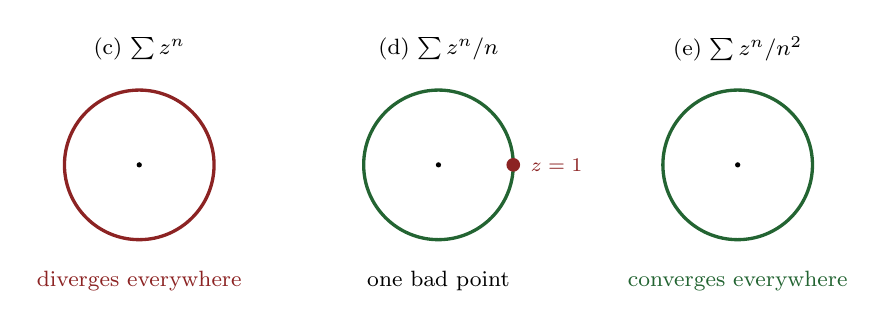
\begin{tikzpicture}[scale=0.95]
    % (c) diverges everywhere
    \begin{scope}[shift={(0,0)}]
      \node at (0,1.55) {\footnotesize (c) $\sum z^n$};
      \draw[very thick, thmcolor] (0,0) circle (1);
      \fill (0,0) circle (1pt);
      \node[thmcolor] at (0,-1.55) {\footnotesize diverges everywhere};
    \end{scope}
    % (d) one bad point
    \begin{scope}[shift={(4,0)}]
      \node at (0,1.55) {\footnotesize (d) $\sum z^n/n$};
      \draw[very thick, proofcolor] (0,0) circle (1);
      \fill (0,0) circle (1pt);
      \fill[thmcolor] (1,0) circle (2.6pt);
      \node[thmcolor, right] at (1.1,0) {\scriptsize $z = 1$};
      \node at (0,-1.55) {\footnotesize one bad point};
    \end{scope}
    % (e) converges everywhere
    \begin{scope}[shift={(8,0)}]
      \node at (0,1.55) {\footnotesize (e) $\sum z^n/n^2$};
      \draw[very thick, proofcolor] (0,0) circle (1);
      \fill (0,0) circle (1pt);
      \node[proofcolor] at (0,-1.55) {\footnotesize converges everywhere};
    \end{scope}
  \end{tikzpicture}
  \end{center}

  \vspace{0.4em}
  \begin{center}
    \hl{\textbf{Same radius $R = 1$ --- yet \alert{three different} boundary behaviors.}}
  \end{center}

  \note{
    Here are the three radius one examples side by side, each drawn as the
    unit circle in the complex plane. On the left, example "c", the plain
    geometric series: the whole circle is red, because the series diverges
    at every point of the boundary. In the middle, example "d", the series
    of "z" to the "n" over "n": the circle is green, meaning it converges,
    except for one red dot at "z" equals one, where it becomes the harmonic
    series and diverges. That is the single bad point. On the right, example
    "e", with "n" squared in the denominator: the whole circle is green, so
    it converges everywhere. The lesson is striking. All three have exactly
    the same radius of convergence, one, yet the behavior on the boundary
    tells three completely different stories. Next, let's summarize.
  }
\end{frame}

}

{
\usebackgroundtemplate{%
  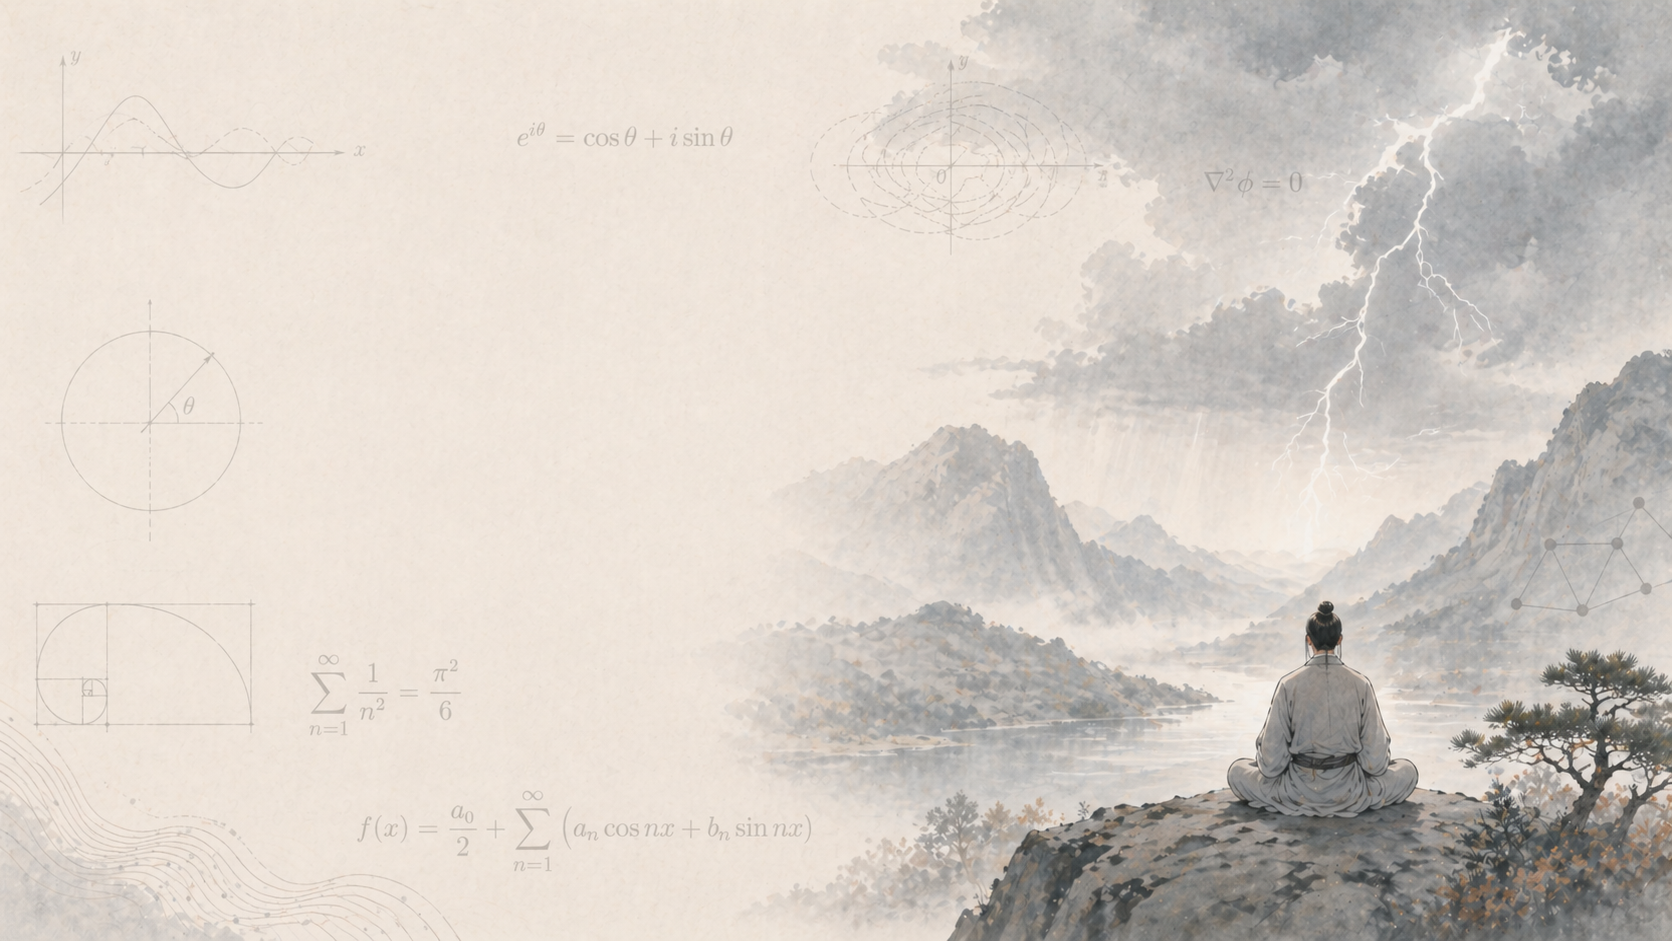
\includegraphics[width=\paperwidth,height=\paperheight,keepaspectratio=false]{chapter_03_bg_05.png}%
}
% =============================================================================
\section{Summary}
% =============================================================================

% --- Build 1/2 ---
\begin{frame}{Summary}
  \begin{hlbox}
    \textbf{Key takeaways:}
    \begin{itemize}
      \item \alert{Definition 3.38:} a power series is $\sum c_n z^n$
      \item \alert{Theorem 3.39:} with $\alpha = \limsup\sqrt[n]{|c_n|}$ and
        $R = 1/\alpha$, the series converges for $|z| < R$, diverges for $|z| > R$
    \end{itemize}
  \end{hlbox}

  \note{
    Let's gather the key ideas. First, a power series is an infinite sum
    of coefficients "c" sub "n" times powers of a complex variable "z".
    Second, and most importantly, the radius of convergence "R" is one
    over alpha, where alpha is the limit superior of the "n"th root of the
    absolute value of the coefficients. Inside the disk of radius "R" the
    series converges; outside it diverges. This number is read directly
    off the coefficients, with no reference to "z". Next, the part the
    theorem leaves open.
  }
\end{frame}

% --- Build 2/2 ---
\begin{frame}{Summary}
  \begin{hlbox}
    \textbf{Key takeaways:}
    \begin{itemize}
      \item \alert{Definition 3.38:} a power series is $\sum c_n z^n$
      \item \alert{Theorem 3.39:} with $\alpha = \limsup\sqrt[n]{|c_n|}$ and
        $R = 1/\alpha$, the series converges for $|z| < R$, diverges for $|z| > R$
      \item On the circle $|z| = R$: behavior \alert{varies} (examples c, d, e)
    \end{itemize}

    \vspace{0.8em}
    \textbf{Coming up next:} Summation by Parts.
  \end{hlbox}

  \note{
    Third, the theorem is silent about the boundary circle itself, where
    the absolute value of "z" equals "R", and for good reason. Our three
    radius one examples showed every possibility: divergence at all
    boundary points, divergence at just one point, and convergence
    everywhere on the circle. Settling these delicate boundary cases
    requires a new tool. That tool is summation by parts, the subject of
    the next section, which will let us prove the convergence claims we
    had to postpone. See you there.
  }
\end{frame}
}

\end{document}
